\documentclass[journal]{IEEEtran}
\usepackage[utf8]{inputenc}
\usepackage{amsmath}
\usepackage{amsfonts}
\usepackage{amssymb}
\usepackage{graphicx}
\usepackage[left=2cm,right=2cm,top=2cm,bottom=2cm]{geometry}
\usepackage[export]{adjustbox}
\usepackage{subfigure,color,amsmath,amssymb,amsfonts}
\usepackage{url,graphicx,subfigure}

% Some handy Latin commands
\newcommand{\etal}{\textit{et al}.}
\newcommand{\ie}{\textit{i}.\textit{e}.,}
\newcommand{\eg}{\textit{e}.\textit{g}.}

\begin{document}
\title{Decoding of a Simple CDMA System}
\author{Alon S. Levin\thanks{The Cooper Union, Department of Electrical Engineering}\\Wireless Communications\\ECE-408 --- Spring 2020}
\maketitle

\begin{abstract}

\end{abstract}

\begin{IEEEkeywords}
CDMA, Walsh channel, M-sequences, despreading
\end{IEEEkeywords}

%%%%%%%%%%%%%%%%%%% Introductions %%%%%%%%%%%%%%%%%%
\section{Introduction}\label{sec:intro}
Code-Division Multiple Access (CDMA) is a channel access method allowing multiple users to communicate across the same spread-spectrum channel. A simple CDMA system was proposed by Prof. Hoerning for the purpose of this assignment.

The transmitter of the simple CDMA system can be seen in Fig.~\ref{fig:transmitter}. A BPSK-encoded message is orthogonally spread on Walsh channel 5 using an 8-ary Hadamard transform; a pilot message consisting of all zeros is likewise encoded and spread on Walsh channel 0. An $8^{\text{th}}$ order M-sequence with an unknown offset is used to spread the signal, after which the signal is $4\times$ oversampled, baseband filtered with an FIR root raised cosine (RRC) filter, and up-converted.

The unencoded message is composed of $N$ total frames, in which the first and last frames contain the pilot signals only. Each frame contains 255 chips; each set of 64 chips represents an ASCII character. Therefore, each frame represents at most three ASCII characters. This is shown in Fig.~\ref{fig:message}.

Each student received an individualized transmission created using this system, and it was his or her task to decode the signal and interpret the hidden ASCII message. In addition to standard decoding, the signal was impaired by unknown frequency and phase offsets that required compensation.

\begin{figure}[!htbp]
    \centering
    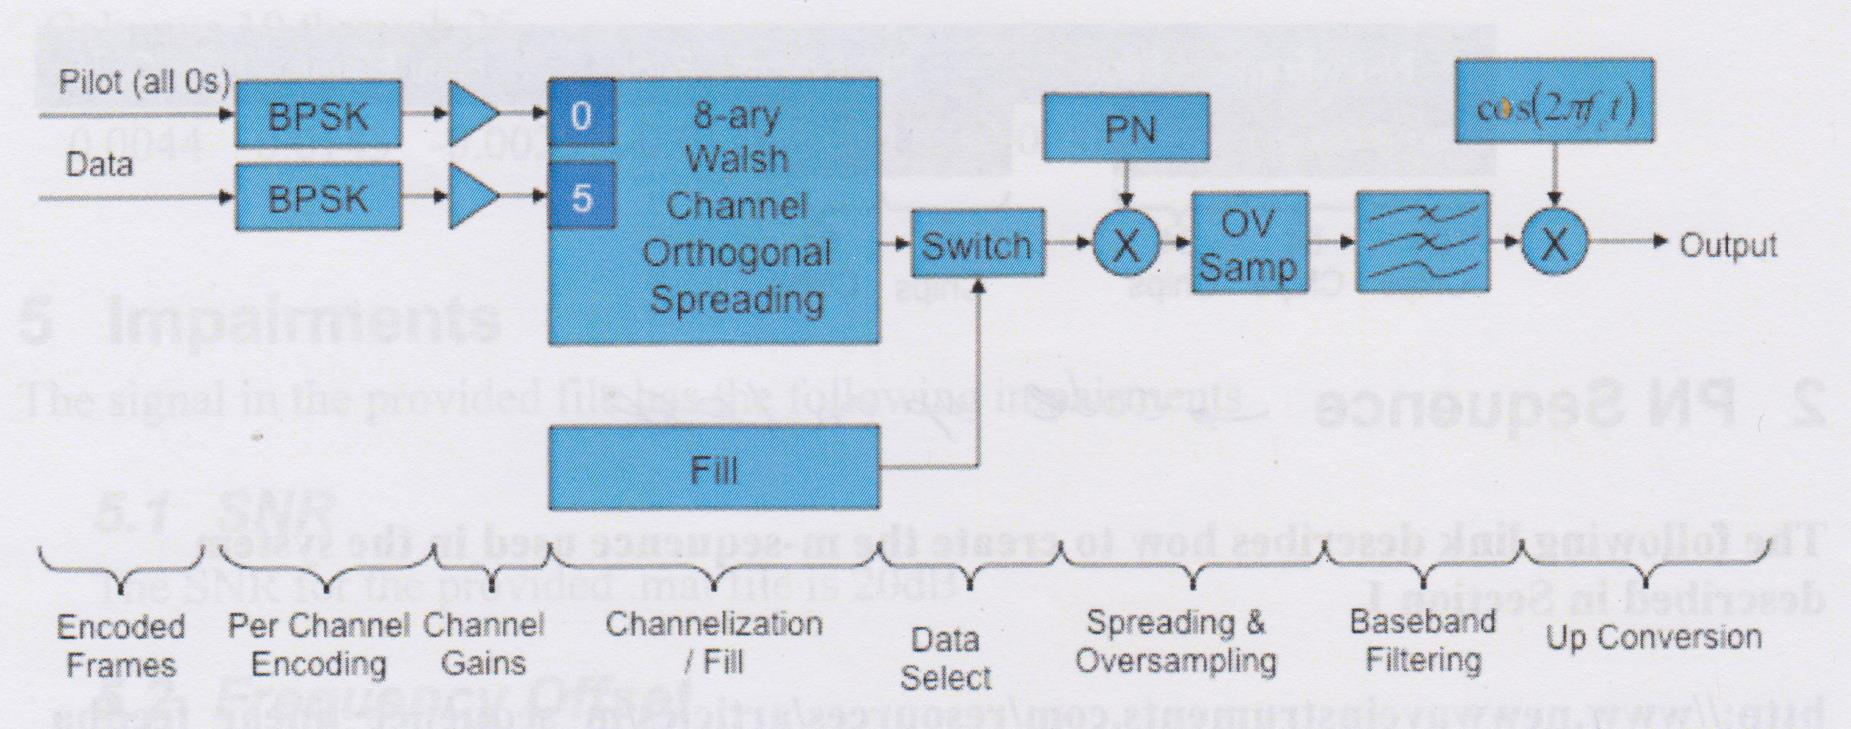
\includegraphics[width = 0.45\textwidth]{CDMA_transmitter.jpg}
    \caption{Simple CDMA transmitter.}
    \label{fig:transmitter}
\end{figure}

\begin{figure}[!htbp]
    \centering
    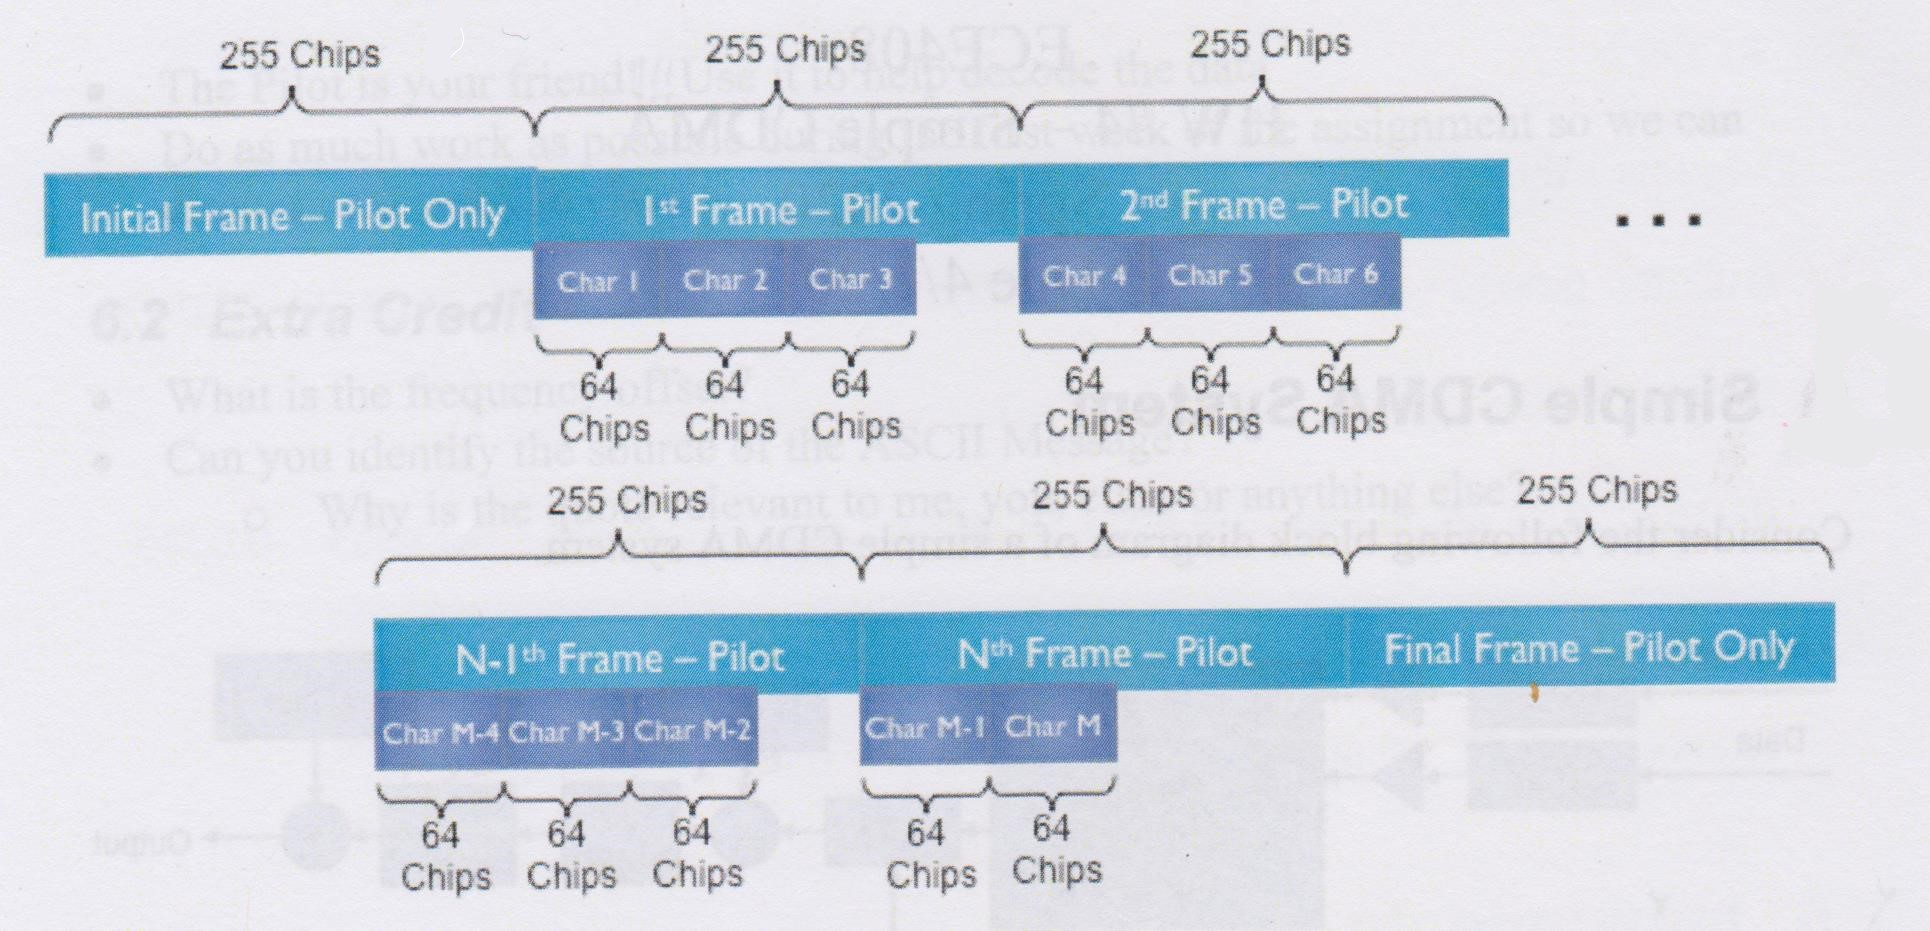
\includegraphics[width = 0.45\textwidth]{CDMA_sig.jpg}
    \caption{Composition of a message transmitted using this system.}
    \label{fig:message}
\end{figure}

\section{CDMA Decoding Process} \label{sec:decoder}
To decode the signal, a backwards process was used to undo each of the transmitter's steps sequentially. First, the received signal was filtered with the RRC and $4\times$ downsampled, resulting in a signal consisting of 33 frames. 

The next step was to determine the correct M-sequence used. An LFSR was generated and shifted according to a set of taps that mirror those used in the transmitter, determined using the following formula:
\begin{equation}
	\vec{\tau}_m = \{\tau[0], \tau[0] - \tau[1], \tau[0] - \tau[2], \ldots\}
\end{equation}

The cross-correlation between a 255-length M-sequence and the real component of first frame of the signal was used to determine the offset in the M-sequence, which was simply the index of the maximum cross-correlation. Thus, we now obtained the starting point in the signal, and could now determine where the first and final pilot frames were located.

By extracting and demodulating these frames, we could estimate the phase and frequency offsets that were affecting the signal. Offets were calculated for each of the two frames, and the median was taken as the ``average'' value used for correcting the data-carrying frames of the signal. The signal before and after frequency shift correction can be seen in Fig.~\ref{fig:freqshift}.

\begin{figure}[!htbp]
    \centering
    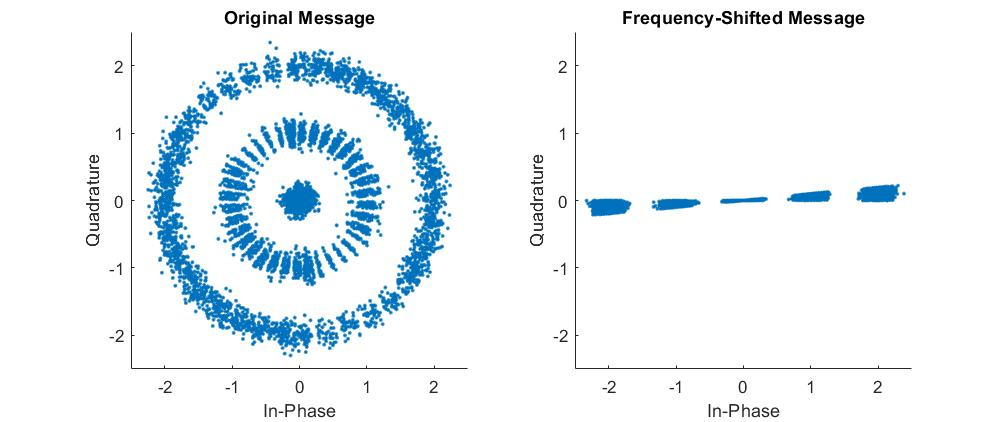
\includegraphics[width = 0.45\textwidth]{freq_shift.jpg}
    \caption{Received signal, before and after frequency reshifting.}
    \label{fig:freqshift}
\end{figure}

The reshifted frames still contained pilot information, however, that was transmitted on Walsh channel 0. All-zero pilots were encoded, transmitted through the Walsh channel, and spread with the M-sequence. The resulting signal was then cancelled from the reshifted frames, thereby obtaining frames that contained data only. The pilot-cancelled signal can be seen in Fig.~\ref{fig:nopilots}.

\begin{figure}[!htbp]
    \centering
    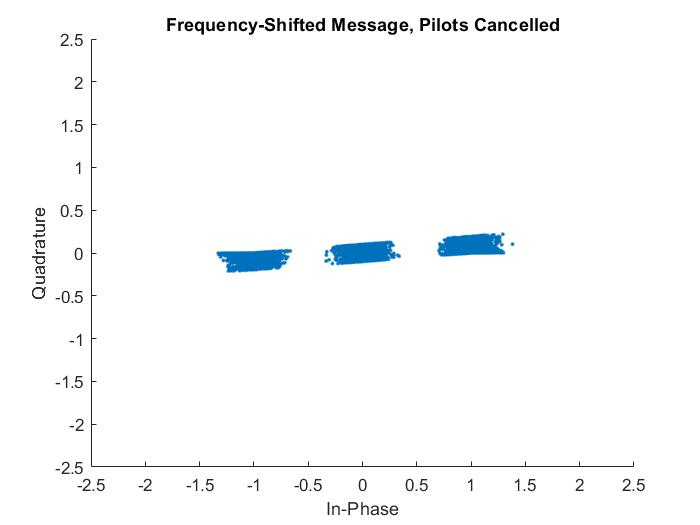
\includegraphics[width = 0.45\textwidth]{nopilots.jpg}
    \caption{Frequency-corrected signal after pilot cancellation.}
    \label{fig:nopilots}
\end{figure}

Note that not all chips represented characters in the signal; it is for this reason that there are symbols about the origin in the previous figure. The task, now, is to remove these non-character symbols before BPSK demodulation takes place. The signal was reshaped from a single vector to a matrix in which each column vector represented a single frame. The first $3\times64$ chips were kept in each frame, and the rest discarded. This is sufficient to clean all data frames but the last, as we do not know how many characters were transmitted in the final data frame. To solve this, the matrix was once again reshaped such that each column represented a single character; all columns in which all real components had a magnitude less than 0.5 were presumed to be ``false'' characters and removed.

Finally, the resulting signal was despread with the M-sequence and Walsh channel 5, BPSK-demodulated, and translated from binary to ASCII succesfully.

\section{Results \& Discussion}
The frequency offset was found to be approximately 108.987028 Hz. The phase offset was found to be approximately -44.695325$\deg$. The secret message was  
\begin{quote}
\emph{Let me give you a piece of advice, junior: your music make sense to no one... but yourself.}
\end{quote}

What is the meaning of this quote? In fact, it is multifaceted:
\begin{itemize}
\item This is a quote from Prince's film \emph{Purple Rain} (1984).
\item I first met Prof. Hoerning when I took his ``Music \& Engineering'' class as a Junior.
\item I have shown him many strange songs (see: Eurovision) that quite often simply don't make sense to those unfamiliar to them.
\end{itemize}

%%%%%%%%%%%%%%%%%%% Bibliography %%%%%%%%%%%%%%%%%%%
\bibliographystyle{unsrt}
%% To reload citations:
%% F6 --> F11 --> F6 --> F6 --> F7
\bibliography{Bibliography} %filename (no .bib)

\end{document}